\documentclass[12pt,a4paper,twoside]{article}

\usepackage[english]{babel}

%------------------------------ encoding
\usepackage[utf8]{inputenc}
\usepackage{csquotes}

%------------------------------ page layout
\usepackage[left=3cm,right=3cm,top=3cm,bottom=2cm]{geometry}

%------------------------------ clickable toc and links styles
\usepackage{hyperref}
\hypersetup{
    colorlinks,
    citecolor=black,
    filecolor=black,
    linkcolor=black,
    urlcolor=black
}

%------------------------------ font macro
\newcommand*{\courierfont}{\fontfamily{pcr}\selectfont}

%------------------------------ references
\usepackage{biblatex}
\addbibresource{bib.bib}

%------------------------------ tables
\usepackage{tabularx}

%------------------------------ images
\usepackage{graphicx}

%------------------------------ font preferences (1) or sc
\usepackage[sc]{mathpazo} 
% \usepackage{newpxmath}

%------------------------------ comment
\usepackage{comment}

%------------------------------ title spec
\usepackage{titlesec}
\usepackage{afterpage}

%------------------------------ abstract
\usepackage{abstract}
\renewcommand{\abstractnamefont}{\normalfont\Large\bfseries}

%------------------------------ page numbering
\usepackage{lastpage}
\usepackage{fancyhdr}
\pagestyle{fancy}
\fancyhf{}
\fancyfoot[R]{\thepage \hspace{1pt} of \pageref{LastPage}}

\begin{document}

\begin{comment}
\begin{titlepage}
    \centering
    \vspace*{\fill}

    \vspace*{0.5cm}
    
    \huge ACULEI
    
    \vspace*{2.5cm}
    
    \vspace*{1cm}

    \begin{minipage}{\textwidth}
        \centering
        \begin{tabular}{ccc}
            \small \textbf{Brajucha Filippo} & \small \textbf{Dinelli Michele} & \\
            \small University of Bologna & \small University of Bologna & \\
            \scriptsize \courierfont{\href{mailto:filippo.brajucha@studio.unibo.it}{filippo.brajucha@studio.unibo.it}} & \scriptsize \courierfont{\href{mailto:michele.dinelli5@studio.unibo.it}{michele.dinelli5@studio.unibo.it}} & \\
        \end{tabular}
    \end{minipage}

    \vspace*{1cm}

    \begin{minipage}{\textwidth}
        \centering
        \begin{tabular}{ccc}
            \small \textbf{Hanna Youssef} \\
            \small University of Bologna \\
            \scriptsize \courierfont{\href{mailto:youssefawni.hanna@studio.unibo.it}{youssefawni.hanna@studio.unibo.it}} \\
        \end{tabular}
    \end{minipage}
    
    \vspace*{\fill}
\end{titlepage}

\tableofcontents

\newpage

\end{comment}

\begin{center}

\rule[0.1cm]{15.8cm}{1.5mm}
{{\Large{Aculei}}} 
\rule[0.1cm]{15.8cm}{0.1mm}

\vspace*{1cm}

\begin{minipage}{\textwidth}
    \begin{tabular}{ccc}
        \small \textbf{Brajucha Filippo} & \small \textbf{Dinelli Michele} & \small \textbf{Hanna Youssef} \\
        \small University of Bologna & \small University of Bologna & \small University of Bologna \\
        \scriptsize \texttt{\href{mailto:filippo.brajucha@studio.unibo.it}{filippo.brajucha@studio.unibo.it}} & \scriptsize \texttt{\href{mailto:michele.dinelli5@studio.unibo.it}{michele.dinelli5@studio.unibo.it}} & \scriptsize \texttt{\href{mailto:youssefawni.hanna@studio.unibo.it}{youssefawni.hanna@studio.unibo.it}} \\
    \end{tabular}
\end{minipage}

\vspace*{1cm}
    
\end{center}

\begin{abstract}    
\noindent This report describes the steps in the process of building a dataset that collects data from photographs of animals taken automatically by photo-traps located in the forests of Umbria. Realizing the dataset aims to collect a vast amount of data, so as to put it at the service of artificial intelligence techniques in order to group and potentially classify the photographs. \\ Two approaches are explored: the first involves unsupervised learning based on algorithms of clustering, while the second is based on a technique called \textit{zero-shot image classification} in order to classify photographs according to the animal portrayed. \\ 
In recent years, the discipline known as computer vision has made enormous strides, thanks to this branch of computer science it is possible to manipulate complex data, such as photographs, extracting knowledge from them. The information obtained from photographs, the relationships and hidden patterns that are identified by artificial intelligence are used to generate an interactive experience within a photographic archive called \textit{aculei}. The project \textit{aculei} is the brainchild of a Milanese photographer who placed several automatic photo-traps in the woods surrounding the house in which he grew up in Umbria. The desire to publish the photographs and make the experience on the archive ai-driven are his motivations for conceiving the project \textit{aculei}.
\end{abstract}

\section{Introduction}
Computer vision is a field of artificial intelligence that allows computers to extract 
information and data from digital images, videos and other visual inputs. It works in much the same way as human vision, but humans have a great advantage: they have years and years of experience in which they they have trained themselves to distinguish objects \cite{ibm-comp-vision}. Computers have to do the same but in much less time by generally resorting to deeplearning techniques by exploiting a type of neural networks known as convolutional neural networks. Several techniques have been used based on computer vision such as ocr (optical character recognition) \footnote{is a term that describes the programs dedicated to optical character recognition in a document} and zero-shot image classification \footnote{a computer vision task for classifying images into a given class, without any training or prior knowledge of the classes}. \\ Computer vision was extensively exploited to realize the spines dataset since the data provided are more than 16000 digital images that must necessarily be processed by a computer.

\begin{figure}[!ht]
    \centering
    \includegraphics[width=\textwidth ,height=\textheight, keepaspectratio]{assets/TF_ACULEI_16567_DSCF0121.jpg}
    \caption{Example of a digital image taken by one of the photo-traps}
    \label{fig:TF_ACULEI_16567_DSCF0121}
\end{figure}

\subsection{Description of the problem}
You want to create a dataset containing data from photographs taken automatically from photo-traps 
placed in Umbria. The photographs were made available by the photographer owner of the 
photo-traps who has been collecting them for the past 4 years.\\
From the photographs we want to extract key data such as temperature, moon phase, the camera 
that took the image, and the date and time. Very ambitious is the recognition of the animal portrayed. Photographs may contain among the meta-data some of this information while some times it is completely absent such as temperature measurement and information on the type of 
animal. The loss of some information in the meta-data could be caused by intermediate software 
that the photographer used to process the photos before providing them for the study.\\ 
The problem then is to define a set of procedures for processing the images, extracting from them the relevant information and then create a dataset on which to apply artificial intelligence techniques to identify correlations among the photographs so as to provide an immersive experience on the archive photograph that collects them.

\subsubsection{Problem rationale and relevance}
The spines project stems from the desire of the photographer who owns the photo-traps to make public photographs. To do so, he wanted to initiate the development of an online photo archive with a strong artistic imprint. \\ In addition to studies stylistics related to interaction and user experience, a phase has been planned in which artificial intelligence is applied so that it guides the user experience on the archive. In the context of the aculei project, the phase described in this paper represents a very important point in the development of the backend system related to the photo archive.

\subsubsection{Interested audience}
People interested in this project are those who want to observe the various stages of creating 
of a dataset from data collection to the creation of the complete dataset. In addition, 
those who want to use the dataset for their own studies or expand 
and improve those at the moment carried out.

\subsubsection{Benefits of a solution}
A detailed and well-documented solution is certainly helpful in defining the steps needed to 
creation of a dataset in the most correct and meaningful way, highlighting the difficulties and strengths. \\ Making a satisfactory, orderly, and easily usable dataset also means completing the 
component that manages the interaction on the archive \textit{aculei} through the website, then 
create a platform for displaying this photographic content, making the most of its 
features. 

\subsection{Proposed Solution}

\subsubsection{Approach to the solution}
The first idea was to develop an artificial intelligence with the available images. The artificial intelligence in question would have to predict the next image to recommend to the user from the previously recommended images. The process turned out to be rather complex because of the nature of the data (high-resolution images that had to be pre-processed in a precise manner). Under the circumstances, the idea was abandoned and we focused on an unsupervised approach based on clustering algorithms. To arrive at clustering processes, however, the basis remains the creation of a dataset on which to apply unsupervised learning. \\ For the purpose of building a dataset from digital photographs, we first asked ourselves what data were present and therefore extractable from a digital photograph. As can be seen in figure \ref{fig:TF_ACULEI_16567_DSCF0121} the photographs in question have a black horizontal stripe showing some of the meta-data exported directly from the photo-trap at the time it was taken. The meta-data are: the photo-trap that took the photo (camera), moon phase, temperature, date and time. This situation introduces two problems to consider: the horizontal strip of meta-data is not always present in the photographs (for reasons not currently determined) and the meta-data are not also found in the file meta-data, they are only present in the image in the form of pixels. Given these two issues, two steps were identified in order to accurately extract meta-data from the images: meta-data reading and extraction using \textit{Exiftool} \cite{exiftool} and ocr techniques using python libraries such as \textit{PyTesseract} \cite{pytesseract} and \textit{EasyOCR} \cite{easyocr} to extractg text from images. Once the two steps were carried out, a primitive version of the dataset was obtained but rich in infromations from which knowledge could be extracted.

\subsubsection{IT challenges faced}
The main problems encountered are related to the quality of the images (not always optimal) and the unevenness of the data. For example, in some cases some meta-data were successfully extracted using \textit{Exiftool} while in other cases they were not. We had to provide fallback cases so that no information was lost. Another obstacle was time; in fact, applying ocr to photographs was not computationally fast. Some sort of pre-processing had to be provided to decrease the number of pixels that the libraries had to consult by cropping the photographs. This pre-processing added to the actual time to extract text from the images caused several takes. We used two libraries because comparing we noticed that the best results were obtained combining and merging the two outputs. \\ Another problem faced had to do with the encoding of the dataset, which is rich in categorical variables. We had to go very deep into these terms. As well as we had to delve into how we would choose the number of clusters and how to use the dataset for unsupervised learning (PCA analysis). Another challenge faced stems from the ambition we had in wanting to extract the label of the portrayed subject from the images as well. This caused a lot of time spent and we tried numerous approaches, evaluating for various pre-designed models without fine-tuning. Finally we agreed to the use of zero-image-classification of huggingface \cite{huggingface}.

\subsubsection{SOA - State of the art}
TODO

\subsubsection{Group management}
The group worked fairly evenly in the implementation of the project, all of them having 
participated in different ways in its completion.\\ During the writing of the code, an approach in which everyone was free to criticize and advise what was the ideal solution for him. There were many situations where we got together and tried to devise and develop ideas so that we could 
solve the problems encountered along the way.
% \textit{DA ESTENDERE}

\subsubsection{Results obtained - a summary}
We obtained a dataset from photos of animals taken by photo-traps. Each row in the dataset has information at the time of the shot such as moon phase, datetime, the most likely label of the subject pictured, a unique identifier, temperature, and season, and the photo-trap that took it. Some data are derivable but still useful for unsupervised learning tasks.

\newpage
\section{Metodo Proposto}
Il metodo proposto è un insieme di differenti metodi che abbiamo testato durante l'esecuzione
per trovare quale fosse la soluzione più adeguata alle nostre esigenze.\\
Si può dire quindi che abbiamo esplorato una ampio spazio delle soluzioni per giungere a quella 
che ci sembrava essere la soluzione ideale.

\subsection{Scelta della Soluzione}
La soluzione scelta è stata quella di creare un percorso interattivo tra immagini correlate in 
grado di coinvolgere e stupire l'utente in modo dinamico. Questa soluzione è stata ottenuta 
eseguendo la clusterizzazione delle immagini raccolte.\\
Una volta collezionate, le fotografie, sono state categorizzate e indicizzate in modo da creare 
un dataset di partenza contenente tutte le informazioni reperibili più facilmente, in modo da 
poterle studiare e ordinare per poi proporre un percorso interessante all'utente finale.\\
Le soluzioni proposte non sono state poche, abbiamo provato diversi metodi e testato diverse 
tecnologie per ottenere il risultato migliore, quello che coincidesse esattamente con le nostre 
necessità di avere un sistema reattivo e sempre pronto ad essere aggiornato e migliorato con 
altre immagini e informazioni, personalizzabile dall'utente e utile sia come intrattenimento, 
quindi a scopo ludico, che interessante dal punto di vista scientifico e dell'osservazione. Per 
questo abbiamo studiato e ci siamo anche informati su quali potessero essere le correlazioni 
scientifiche con ciò che osservavamo e ciò che valutavamo, in modo da poter avere anche un 
occhio critico per poter valutare se i risultati scovati fossere corretti oppure inutili e 
sbagliati. Non essendo una materia di nostra competenza, infatti, abbiamo dovuto prestare molta 
attenzione.\\
La soluzione corretta è stata scelta anche dopo aver effettuato dell'inferenza sui dati in modo 
da osservare la distribuzione degli stessi e capire se ci fossero stati dei problemi. 

\subsubsection{Alternativi considerati e giustificazioni della scelta}
Per realizzare un percorso esplorativo tra leimmagini abbiamo fin da subito provato a realizzare 
un'AI in grado di riconoscere l'animale selvatico dall'immagine selezionta, una sorta di 
\texttt{lens} in grado di analizzare la foto e il contesto per poter tracciare quale fosse il 
soggetto e collegarla ad altre fotografie simili. L'idea è stata abbandonata piuttosto 
velocemente perchè le risorse a disposizione erano molto inferiori a quelle richieste da un 
lavoro così costoso computazionalmente parlando.\\
Per questo abbiamo optato per una soluzione più alla nostra portata e ugualmente molto 
interessante, abbiamo creato un dataset con le immagini a nostra disposizione abbiamo provato 
ad utilizzare diversi metodi di clusterizzazione con diversi parametri.\\
Dopo diverse prove e ricerche abbiamo capito che solo empiricamente e provando si può ottenere 
il risultato migliore e più adatto alle esigenze, seguendo anche la letteratura di riferimento.\\
Una volta eseguito il clustering siamo tornati sui nostri passi e abbiamo testato un metodo di 
\textit{zero-shot image classification} per poter classificare gli animali, siamo così riusciti 
ad ottenere dei risultati molto soddisfacenti.

\subsubsection{Metodologia per la misurazione delle performance}
La misurazione della performance è avvenuta tramite diversi metodi e in diversi momenti durante la 
realizzazione di questo progetto. Abbiamo sempre cercato di ottenere dei buoni risultati tenendo 
sotto controllo i dati ottenuti.\\
Per questo motivo, durante la creazione del dataset, abbiamo effettuato diversi test e diverse 
misurazioni per vedere se i dati in output fossero sensati e collezionati nel modo corretto senza 
particolari incongruenze.\\
Per il nostro progetto risulta molto complesso parlare di misurazione della performance visto che 
il risultato proposto è soggettivamente buono e non può essere valutato da parametri numerici. 
Generalmente possiamo osservare che i risultati proposti sono di nostro gradimento ma sicuramente 
possono esserci delle personalizzazioni che magari cambiano l'output in modo da ottenerne uno più 
utile al proprio scopo, magari modificando le varibili della clusterizzazione o il numero di 
clusters.\\
% \textit{DA ESTENDERE / RIVEDERE}


\newpage
\section{Risultati Sperimentali}

\subsection{Dimostrazione e Tecnologie}

\subsubsection{Istruzione per la dimostrazione}
La dimostrazione che si ottiene non è altro che un percorso tra delle immagini che sono 
evidentemente correlate. Il percorso di selezione delle features, e in generale di setting di 
tutto il sistema di clusterizzazione, è avenuto dopo uno studio del dataset basato 
sull'analisi delle componenti principali (\textit{PCA}).\\ 

\subsubsection{Tecnologie e versioni usate (riproducibilità)}
Le immagini sono state scattate e raccolte maualmente da alcune foto-trappole, convertite poi in 
formato \texttt{.jpeg} e caricate su dropbox, tramite il quale è stato possibile lavorare senza 
avere con se la copia fisica delle imamgini stesse.\\ 
Per gli l'algoritmo di clustering è stato utilizzato Python (\textit{Python 3.11.7}) con alcune 
sue librerie per poter gestire e raccogliere i dati, eccone un elenco completo:
\begin{table}[!ht]
    \centering
    \begin{tabular}{||l|r||l|r||}
        \hline
        \textbf{Name} & \textbf{Version} & \textbf{Name} & \textbf{Version} \\
        \hline
        easyocr & 1.7.1 & PyExifTool & 0.5.6 \\
        \hline
        ImageHash & 4.3.1 & pytesseract & 0.3.10 \\
        \hline
        matplotlib & 3.6.0 & pywaffle & 1.1.0 \\
        \hline
        numpy & 1.26.3 & Requests & 2.31.0 \\
        \hline
        opencv\_python\_headless & 4.8.1.78 & scikit\_learn & 1.0.2 \\
        \hline
        pandas & 1.4.3 & seaborn & 0.13.1 \\
        \hline
        Pillow & 10.2.0 & tqdm & 4.65.0 \\
        \hline
        transformers & 4.25.0 & & \\
        \hline
    \end{tabular}
    \caption{Python Libraries Requirements}
\end{table}

\subsection{Risultati}

\begin{table}[!ht]
    \centering
% \setlength{\tabcolsep}{0.5em} % horizontal padding
% {\renewcommand{\arraystretch}{1.5} % vertical padding
    \begin{tabular}{|l|l|l|l|l|}
        \hline
        \textbf{image\_name} & \textbf{camera} & \textbf{date\_time} & \textbf{moon\_phase} & \textbf{temperature} \\ 
        \hline
        a & b & c & d & f\\
        \hline
    \end{tabular}
    \caption{???}
% }
\end{table}

Abbiamo utilizzato i dati presenti nel dataset, ottenuti dall'analisi delle immagini, per 
rappresentare al meglio i risultati ottenuti. Dopo dei processi di inferenza sono stati prodotti 
questi tre grafici, a parer nostro molto significativi al fine di comprendere la distribuzione 
dei dati a nostra disposizione nel tempo. \\
\begin{figure}[!ht]
    \centering
    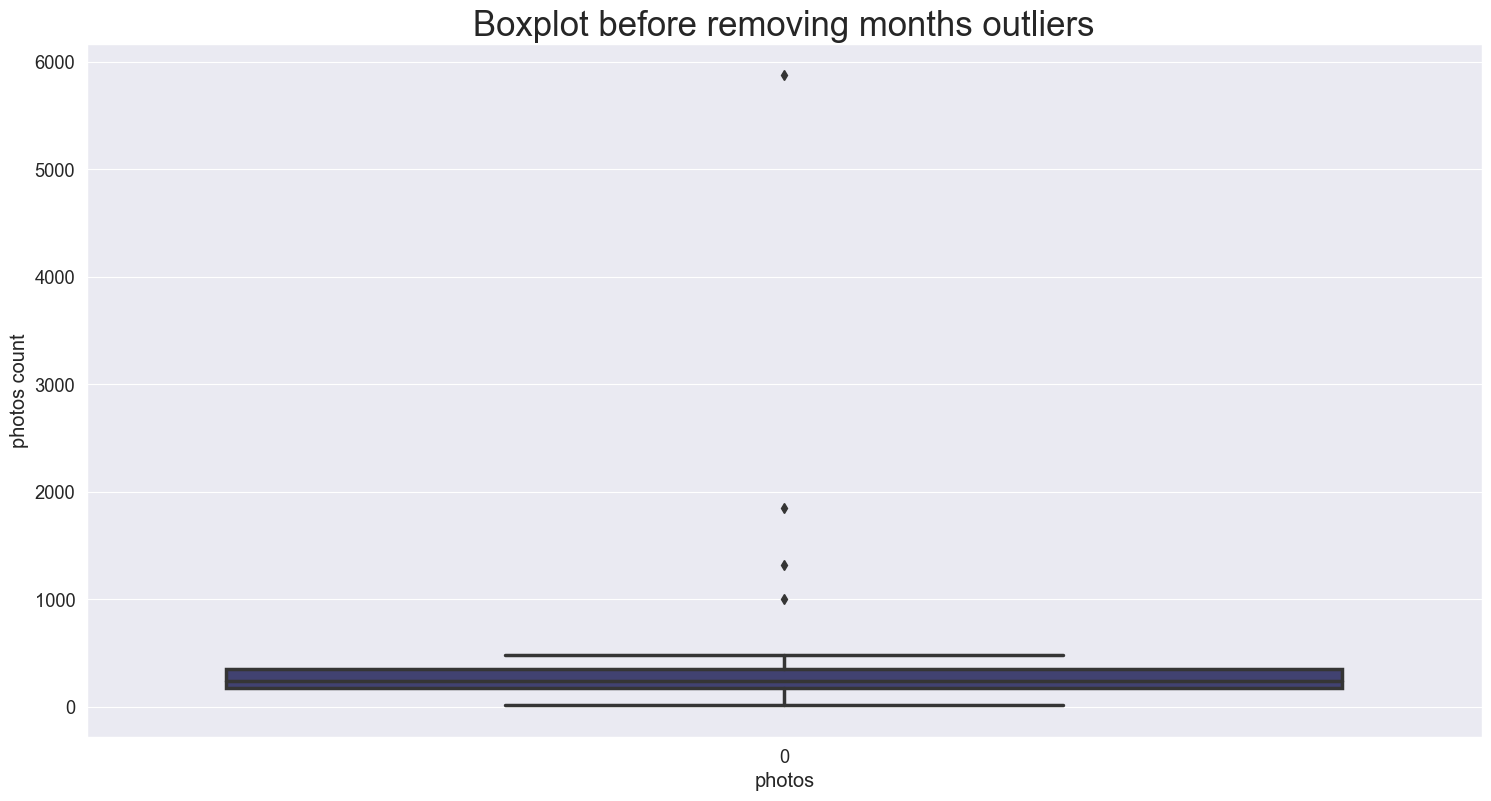
\includegraphics[width=\textwidth, height=\textheight, keepaspectratio]{assets/boxplot-outliers.png}
    \caption{Boxplot dei dati prima di rimuovere gli outliers}
    \label{fig:boxplot-outliers}
\end{figure}
\begin{figure}[!ht]
    \centering
    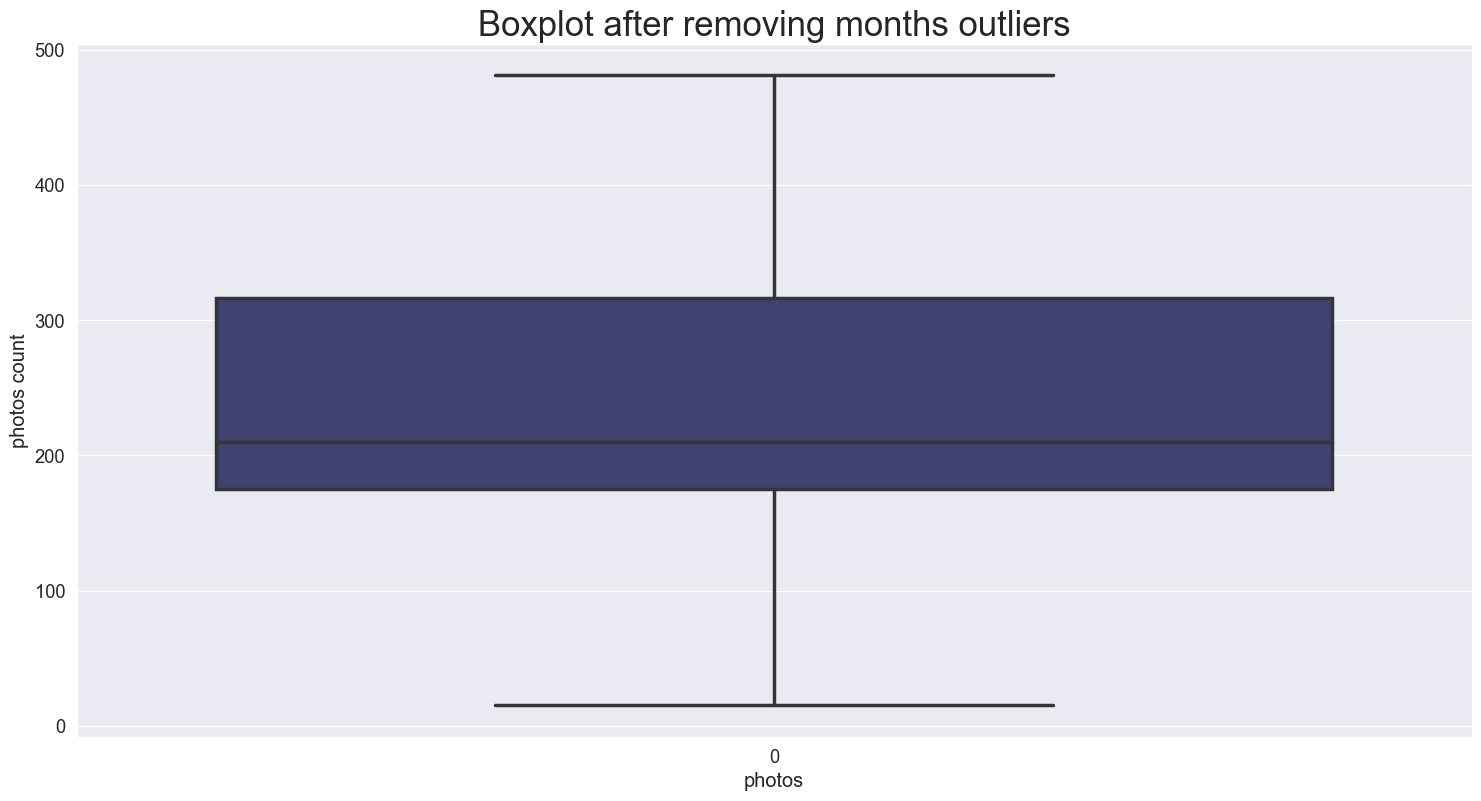
\includegraphics[width=\textwidth, height=\textheight, keepaspectratio]{assets/boxplot-wout-outliers.png}
    \caption{Boxplot dei dati dopo aver rimosso gli outliers}
    \label{fig:boxplot-wout-outliers}
\end{figure}
\begin{figure}[!ht]
    \centering
    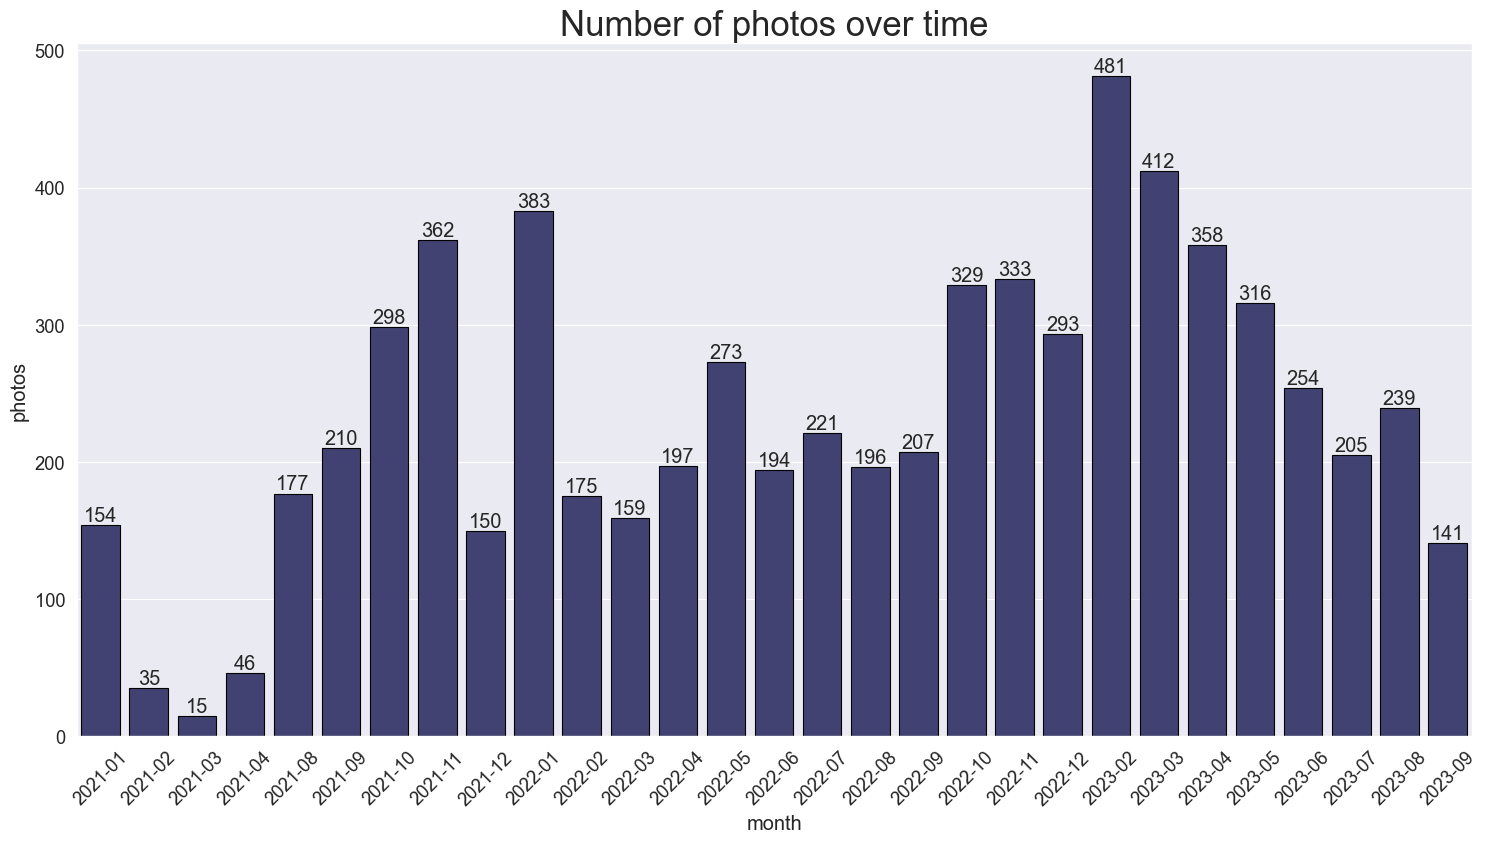
\includegraphics[width=\textwidth, height=\textheight, keepaspectratio]{assets/photos-month.png}
    \caption{Numero totale di fotografie per ogni mese}
    \label{fig:photos-month}
\end{figure}
Il primo grafico è un \textit{boxplot} che rappresenta il numero di foto presenti nel dataset ad 
ogni mese, questo grafico contiene anche i dati etichettati successivamente come 
\textit{outliers}.\\ 
Successivamente abbiamo utilizzato sempre il \textit{boxplot} ma eliminando, appunto, gli 
\textit{outliers} per riuscire a farci un'idea di quante foto effettivamente potevano essere 
scattate in media dalle macchine in un mese.\\
Abbiamo utilizzato i dati senza \textit{outliers} anche per creare un \textit{grafico a barre} 
che fosse più esplitativo sul numero di foto presenti nel dataset suddivise per mese, abbiamo 
comunque osservato che ci sono dei picchi sia molto alti che molto bassi.


\subsubsection{Risultati della configurazione migliore}
Nella configurazione migliore del clustering abbiamo potuto osservare come il nostro sistema 
basato su \textit{zero-shot image classification} fosse comunque molto efficente e ci fornisse 
dei risultati abbastanza soddisfacenti, raggruppando con successo gli animali negli stessi cluster 
oppure comunque con altre immagini effettivamente simili (e quindi correlate).\\ 
% \textit{DA ESTENDERE / RIVEDERE}

\subsubsection{Studio di ablazione: confronto tra configurazioni}
Effetuando la clusterizzazione all'interno del dataset abbiamo affrontato delle scelte che hanno 
comportato delle particolari configurazioni, in particolare abbiamo effettuato la \textit{PCA} e 
abbiamo esaminato i risultati ottenuti grazie alle curve descritte dal variare della varianza in 
base alle components considerate, quella del \textit{Silhouette Score} ed anceh quella del 
\textit{WCSS} (Within-Clusters Sum of Squares).\\
% \textit{DA ESTENDERE / RIVEDERE}
\begin{figure}[!ht]
    \centering
    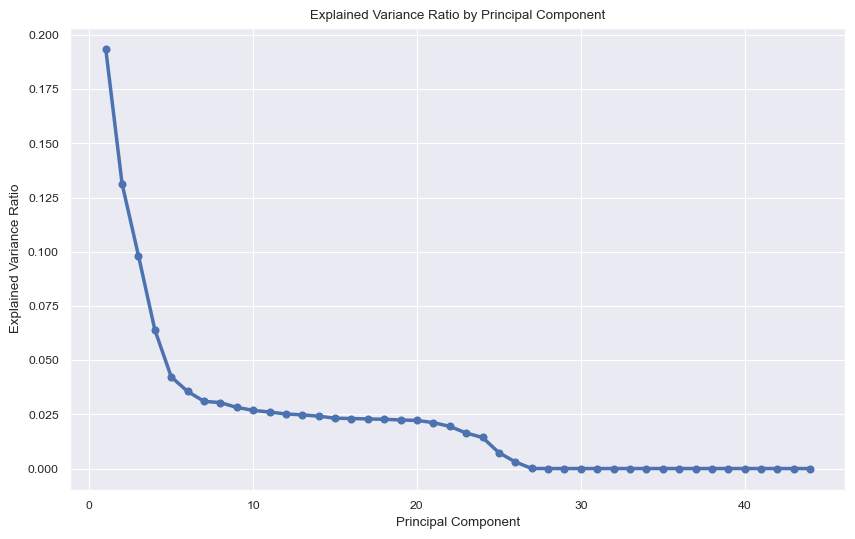
\includegraphics[width=\textwidth, height=\textheight, keepaspectratio]{assets/variance-ratio.png}
    \caption{Rapporto di Varianza per numero di Components Principali}
    \label{fig:variance-ratio}
\end{figure}
\begin{figure}[!ht]
    \centering
    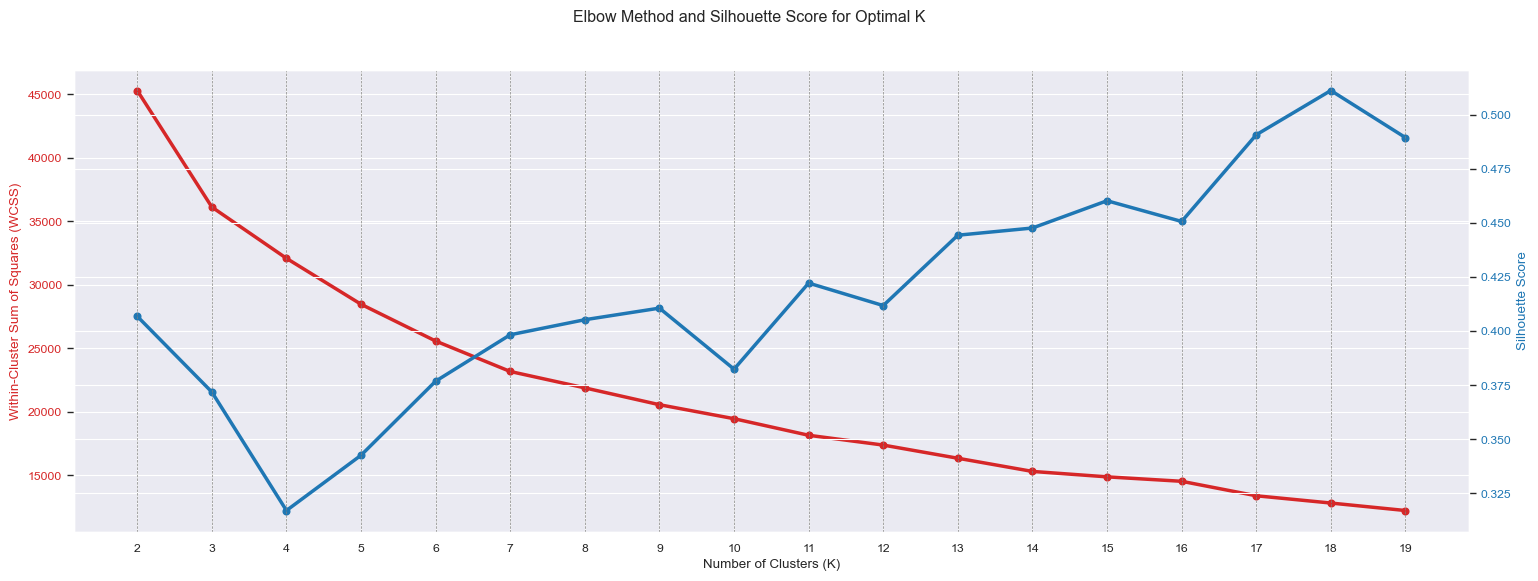
\includegraphics[width=\textwidth, height=\textheight, keepaspectratio]{assets/elbow-silhouette.png}
    \caption{Grafico di comparazione Elbow Method - Silhouette Score}
    \label{fig:elbow-silhouette}
\end{figure}


\subsubsection{Studio di comparazione con letteratura}
% \textit{DA ESTENDERE / RIVEDERE}

\newpage
\section{Discussione e Conclusioni}

\subsection{Discussione dei Risultati}
\subsubsection{Analisi delle performance rispetto alle aspettative}

\subsection{Validità del Metodo}
\subsubsection{Valutazione se il metodo rispetta le aspettative}

\subsection{Limitazione e Maturità}
\subsubsection{Limiti di applicabilità e bias}

\subsection{Lavori Futuri}
\subsubsection{Proposte per avanzare il progetto}

\newpage
\paragraph{Acknowledgements} Si ringrazia Tobia Faverio per aver reso possibile lo sviluppo di 
questo progetto fornendo le fotografie e per la sua idea che ha dato vita ad \textit{aculei}.

\paragraph{Code} available \href{https://gitlab.com/micheledinelli/aculei-ai}{here}

\newpage
\begin{refcontext}[sorting=none]
    \printbibliography
\end{refcontext}

\end{document}